\section{Proof Details}
\label{app:confounding-proofs}

This section organizes the proof material referenced from Chapter~\ref{chap:confounding-test}.

\begin{tcolorbox}[
  enhanced,
  breakable,
  colback=gray!6,
  colframe=chaptercolor,
  boxrule=0.8pt,
  arc=3pt,
  title={Guide to Appendix~\ref{chap:appendix-confounding-test}},
  colbacktitle=chaptercolor!12,
  coltitle=black
]
This appendix is organized in five parts:
\begin{itemize}
  \item proof details for the compatibility lemma, target-effect identification, test validity, and lower-bound validity;
  \item nested trial design and importance-weight identification;
  \item marginal-sensitivity-model tightness and looseness of the lower bound;
  \item experimental details for synthetic, semi-synthetic, and WHI evaluations; and
  \item additional VOTE and Tennessee STAR experiments.
\end{itemize}
\end{tcolorbox}

\subsection{Compatibility of Sensitivity Bounds and Randomized Targets}
\label{app:confounding-proof-compatibility}

This subsection records the proof of Lemma~\ref{lem:confounding-testing-observation}. Under \(H_0(\Gamma)\), the observational full distribution belongs to \(\mathcal{E}(\mathbb{P}^{\mathrm{os}},\Gamma)\). Therefore, by the definition of the CATE sensitivity bounds, for \(\mathbb{P}^{\mathrm{os}}_X\)-almost every \(x\),
\[
  \mu^-_{\Gamma}(x)
  \leq
  \mu(x,\mathbb{P}^{\mathrm{os}}_{\mathrm{full}})
  \leq
  \mu^+_{\Gamma}(x).
\]
Let \(\mathbb{P}_X\) have support contained in \(\supp(\mathbb{P}^{\mathrm{os}}_X)\). If \(\mu(X,\mathbb{P}_{\mathrm{full}})=\mu(X,\mathbb{P}^{\mathrm{os}}_{\mathrm{full}})\) on this support, then the same inequalities hold with \(\mu(X,\mathbb{P}_{\mathrm{full}})\) in the middle. Integrating with respect to \(\mathbb{P}_X\) gives
\[
  \mu^-_{\Gamma}(\mathbb{P}_X)
  \leq
  \mu(\mathbb{P}_X,\mathbb{P}_{\mathrm{full}})
  \leq
  \mu^+_{\Gamma}(\mathbb{P}_X),
\]
which proves the claim.

\subsection{Identification of Target Average Treatment Effects}
\label{app:confounding-proof-ate}

For the randomized-trial target, internal validity gives
\[
\begin{aligned}
  \mu(\mathbb{P}^{\mathrm{rct}}_X,\mathbb{P}^{\mathrm{rct}}_{\mathrm{full}})
  &=
  \mathbb{E}_{\mathbb{P}^{\mathrm{rct}}_{\mathrm{full}}}
  [Y(1)-Y(0)] \\
  &=
  \mathbb{E}_{\mathbb{P}^{\mathrm{rct}}_X}
  \left[
    \mathbb{E}_{\mathbb{P}^{\mathrm{rct}}}[Y\mid T=1,X]
    -
    \mathbb{E}_{\mathbb{P}^{\mathrm{rct}}}[Y\mid T=0,X]
  \right] \\
  &=
  \mathbb{E}_{\mathbb{P}^{\mathrm{rct}}}
  \left[
    Y
    \left(
      \frac{T}{\pi}
      -
      \frac{1-T}{1-\pi}
    \right)
  \right].
\end{aligned}
\]
For the restricted-observational target, transportability of the CATE gives
\[
\begin{aligned}
  \mu(\mathbb{P}^{\widetilde{\mathrm{os}}}_X,\mathbb{P}^{\mathrm{os}}_{\mathrm{full}})
  &=
  \mathbb{E}_{\mathbb{P}^{\widetilde{\mathrm{os}}}_X}
  \left[
    \mathbb{E}_{\mathbb{P}^{\mathrm{os}}_{\mathrm{full}}}
    [Y(1)-Y(0)\mid X]
  \right] \\
  &=
  \mathbb{E}_{\mathbb{P}^{\widetilde{\mathrm{os}}}_X}
  \left[
    \mathbb{E}_{\mathbb{P}^{\mathrm{rct}}_{\mathrm{full}}}
    [Y(1)-Y(0)\mid X]
  \right].
\end{aligned}
\]
Under the absolute-continuity condition \(\mathbb{P}^{\widetilde{\mathrm{os}}}_X\ll\mathbb{P}^{\mathrm{rct}}_X\), with
\[
  w_{\widetilde{\mathrm{os}}}(X)
  =
  \frac{d\mathbb{P}^{\widetilde{\mathrm{os}}}_X}
       {d\mathbb{P}^{\mathrm{rct}}_X}(X),
\]
we obtain
\[
\begin{aligned}
  \mu(\mathbb{P}^{\widetilde{\mathrm{os}}}_X,\mathbb{P}^{\mathrm{os}}_{\mathrm{full}})
  &=
  \mathbb{E}_{\mathbb{P}^{\mathrm{rct}}_X}
  \left[
    \mathbb{E}_{\mathbb{P}^{\mathrm{rct}}_{\mathrm{full}}}
    [Y(1)-Y(0)\mid X]
    w_{\widetilde{\mathrm{os}}}(X)
  \right] \\
  &=
  \mathbb{E}_{\mathbb{P}^{\mathrm{rct}}}
  \left[
    Y
    \left(
      \frac{T}{\pi}
      -
      \frac{1-T}{1-\pi}
    \right)
    w_{\widetilde{\mathrm{os}}}(X)
  \right],
\end{aligned}
\]
where the final equality follows from internal validity (Assumption~\ref{asm:confounding-internal-validity}) and consistency \(Y=Y(T)\). This proves the stated identification formula, with \(w_{\mathrm{rct}}(X)=1\) for the randomized-trial target.

\subsection{Validity of the Statistical Tests}
\label{app:confounding-proof-tests}

First, by definition of the test,
\[
  \{\widehat{\phi}_{\star}(\Gamma,\alpha)=1\}
  \subseteq
  \{\widehat{T}^+_{\Gamma,\star}\leq z_{\alpha/2}\}
  \cup
  \{\widehat{T}^-_{\Gamma,\star}\leq z_{\alpha/2}\}.
\]
It is therefore enough to bound the two one-sided probabilities by \(\alpha/2+o(1)\). We prove this for the upper endpoint; the lower endpoint is analogous.

\paragraph{Case \(\star=\mathrm{rct}\).}
Let
\[
  Z
  =
  \left(
    Y\left(\frac{T}{\pi}-\frac{1-T}{1-\pi}\right),
    \mu^+_{\Gamma}(X)
  \right)^{\top},
\]
with mean
\[
  \left(
    \mu(\mathbb{P}^{\mathrm{rct}}_X,\mathbb{P}^{\mathrm{rct}}_{\mathrm{full}}),
    \mu^+_{\Gamma}(\mathbb{P}^{\mathrm{rct}}_X)
  \right)^{\top}
\]
and covariance matrix
\[
  \Sigma
  =
  \begin{pmatrix}
    \sigma_{\mathrm{rct}}^2 & \xi_{\Gamma,\mathrm{rct}} \\
    \xi_{\Gamma,\mathrm{rct}} & (\sigma^+_{\Gamma,\mathrm{rct}})^2
  \end{pmatrix}
  < \infty,
\]
which is finite because the potential outcomes \(Y(0)\) and \(Y(1)\) are bounded and \(\pi\in(0,1)\). Define
\[
  \bar{\mu}^+_{\Gamma,\mathrm{rct}}
  =
  \frac{1}{n_{\mathrm{rct}}}
  \sum_{X_i\in D_{\mathrm{rct}}}
  \mu^+_{\Gamma}(X_i),
  \qquad
  \Delta^+_{\Gamma,\mathrm{rct}}
  =
  \mu^+_{\Gamma}(\mathbb{P}^{\mathrm{rct}}_X)
  -
  \mu(\mathbb{P}^{\mathrm{rct}}_X,\mathbb{P}^{\mathrm{rct}}_{\mathrm{full}}).
\]
The multivariate central limit theorem implies
\[
  \sqrt{n_{\mathrm{rct}}}
  \left[
    \left(
      \bar{\mu}^+_{\Gamma,\mathrm{rct}}
      -\widehat{\mu}_{\mathrm{rct}}
    \right)
    -
    \Delta^+_{\Gamma,\mathrm{rct}}
  \right]
  \xrightarrow{d}
  \mathcal{N}
  \left(0,V^+_{\Gamma,\mathrm{rct}}\right),
\]
where
\[
  V^+_{\Gamma,\mathrm{rct}}
  =
  (\sigma^+_{\Gamma,\mathrm{rct}})^2
  +
  \sigma_{\mathrm{rct}}^2
  -
  2\xi_{\Gamma,\mathrm{rct}}.
\]
It remains to replace the oracle average of \(\mu^+_{\Gamma}(X_i)\) by \(\widehat{\mu}^+_{\Gamma,\mathrm{rct}}\). Define
\[
  R_n
  =
  \sqrt{n_{\mathrm{rct}}}
  \left(
    \bar{\mu}^+_{\Gamma,\mathrm{rct}}
    -\widehat{\mu}^+_{\Gamma,\mathrm{rct}}
  \right).
\]
If \(d_n(x)=\mu^+_{\Gamma}(x)-\widehat{\mu}^+_{\Gamma}(x)\), then conditional on the observational sample used to train \(\widehat{\mu}^+_{\Gamma}(\cdot)\),
\[
  |\mathbb{E}[R_n\mid D_{\mathrm{os}}]|
  \leq
  \sqrt{n_{\mathrm{rct}}}\|d_n\|_{L^2(\mathbb{P}^{\mathrm{rct}}_X)}
  =
  O_{\mathbb{P}}\!\left(\sqrt{n_{\mathrm{rct}}/n_{\mathrm{os}}}\right)
  =
  o_{\mathbb{P}}(1),
\]
and
\[
  \Var(R_n\mid D_{\mathrm{os}})
  \leq
  \|d_n\|^2_{L^2(\mathbb{P}^{\mathrm{rct}}_X)}
  =
  o_{\mathbb{P}}(1).
\]
By Chebyshev's inequality, \(\mathbb{P}(|R_n|>\varepsilon\mid D_{\mathrm{os}})=o_{\mathbb{P}}(1)\) for every \(\varepsilon>0\). Since \(0\leq\mathbb{P}(|R_n|>\varepsilon\mid D_{\mathrm{os}})\leq 1\), bounded convergence implies \(\mathbb{P}(|R_n|>\varepsilon)=\mathbb{E}[\mathbb{P}(|R_n|>\varepsilon\mid D_{\mathrm{os}})]\to 0\), so \(R_n=o_{\mathbb{P}}(1)\). Slutsky's theorem then gives the same limiting distribution with \(\widehat{\mu}^+_{\Gamma,\mathrm{rct}}\) in place of the oracle average:
\[
  \sqrt{n_{\mathrm{rct}}}
  \left[
    \left(
      \widehat{\mu}^+_{\Gamma,\mathrm{rct}}
      -
      \widehat{\mu}_{\mathrm{rct}}
    \right)
    -
    \Delta^+_{\Gamma,\mathrm{rct}}
  \right]
  \xrightarrow{d}
  \mathcal{N}\bigl(0,V^+_{\Gamma,\mathrm{rct}}\bigr).
\]

By the consistency of the sampling-variance estimators,
\[
\begin{aligned}
  n_{\mathrm{rct}}(\widehat{s}^+_{\Gamma,\mathrm{rct}})^2
  &=
  n_{\mathrm{rct}}(\widehat{\sigma}^+_{\Gamma,\mathrm{rct}})^2
  +
  n_{\mathrm{rct}}\widehat{\sigma}_{\mathrm{rct}}^2
  +
  2\sqrt{n_{\mathrm{rct}}(\widehat{\sigma}^+_{\Gamma,\mathrm{rct}})^2\,n_{\mathrm{rct}}\widehat{\sigma}_{\mathrm{rct}}^2} \\
  &\xrightarrow{p}
  (\sigma^+_{\Gamma,\mathrm{rct}})^2
  +
  \sigma_{\mathrm{rct}}^2
  +
  2\sigma^+_{\Gamma,\mathrm{rct}}\sigma_{\mathrm{rct}}.
\end{aligned}
\]
By Cauchy--Schwarz,
\[
  |\xi_{\Gamma,\mathrm{rct}}|
  \leq
  \sigma^+_{\Gamma,\mathrm{rct}}\sigma_{\mathrm{rct}},
\]
so \(V^+_{\Gamma,\mathrm{rct}} = (\sigma^+_{\Gamma,\mathrm{rct}})^2 + \sigma_{\mathrm{rct}}^2 - 2\xi_{\Gamma,\mathrm{rct}} \leq (\sigma^+_{\Gamma,\mathrm{rct}})^2 + \sigma_{\mathrm{rct}}^2 + 2\sigma^+_{\Gamma,\mathrm{rct}}\sigma_{\mathrm{rct}}\). Because \(z_{\alpha/2}<0\) for all \(\alpha\in(0,1)\), the larger denominator yields a conservative test. Under \(H_0(\Gamma)\), \(\Delta^+_{\Gamma,\mathrm{rct}} = \mu^+_{\Gamma}(\mathbb{P}^{\mathrm{rct}}_X) - \mu(\mathbb{P}^{\mathrm{rct}}_X,\mathbb{P}^{\mathrm{rct}}_{\mathrm{full}}) \geq 0\) by Lemma~\ref{lem:confounding-testing-observation}. Applying Slutsky's theorem together with the asymptotic normality above gives
\[
\begin{aligned}
  &\limsup_{n_{\mathrm{rct}},n_{\mathrm{os}}\to\infty}
  \mathbb{P}_{H_0(\Gamma)}
  \left(
    \widehat{T}^+_{\Gamma,\mathrm{rct}}
    \leq
    z_{\alpha/2}
  \right) \\
  &\quad\leq
  \limsup_{n_{\mathrm{rct}},n_{\mathrm{os}}\to\infty}
  \mathbb{P}_{H_0(\Gamma)}
  \left(
    \frac{
      \sqrt{n_{\mathrm{rct}}}
      \bigl(
        \widehat{\mu}^+_{\Gamma,\mathrm{rct}}
        -
        \widehat{\mu}_{\mathrm{rct}}
        -
        \Delta^+_{\Gamma,\mathrm{rct}}
      \bigr)
    }{
      \sqrt{V^+_{\Gamma,\mathrm{rct}}}
    }
    \leq
    z_{\alpha/2}
  \right) \\
  &\quad=
  \Phi(z_{\alpha/2})
  =
  \alpha/2.
\end{aligned}
\]

\paragraph{Case \(\star=\widetilde{\mathrm{os}}\).}
Let \(n=n_{\mathrm{rct}}+n_{\mathrm{os}}\), with \(n_{\mathrm{rct}}/n\to\rho\in(0,1)\) and hence \(n_{\mathrm{os}}/n\to 1-\rho\). Define
\[
  \sigma_{\widetilde{\mathrm{os}}}^2
  =
  \Var_{\mathbb{P}^{\mathrm{rct}}}
  \left[
    Y
    \left(
      \frac{T}{\pi}
      -
      \frac{1-T}{1-\pi}
    \right)
    w_{\widetilde{\mathrm{os}}}(X)
  \right]
  < \infty,
\]
which is finite since the potential outcomes are bounded, \(\pi\in(0,1)\), and \(\mathbb{E}_{\mathbb{P}^{\mathrm{rct}}}[w_{\widetilde{\mathrm{os}}}(X)^2]<\infty\). By the central limit theorem, Slutsky's theorem, and Appendix~\ref{app:confounding-proof-ate},
\[
  \sqrt{n}
  \left(
    \widehat{\mu}_{\widetilde{\mathrm{os}}}
    -
    \mu(\mathbb{P}^{\widetilde{\mathrm{os}}}_X,\mathbb{P}^{\mathrm{os}}_{\mathrm{full}})
  \right)
  \xrightarrow{d}
  \mathcal{N}(0,\sigma_{\widetilde{\mathrm{os}}}^2/\rho).
\]
Together with the assumed \(\sqrt{n_{\mathrm{os}}}\)-rate asymptotic normality of \(\widehat{\mu}^+_{\Gamma,\widetilde{\mathrm{os}}}\) with limiting variance \((\sigma^+_{\Gamma,\widetilde{\mathrm{os}}})^2\) from Proposition~\ref{prop:confounding-test-validity}(2) and independence of the randomized and observational samples,
\[
  \sqrt{n}
  \begin{pmatrix}
    \widehat{\mu}^+_{\Gamma,\widetilde{\mathrm{os}}}
    -
    \mu^+_{\Gamma}(\mathbb{P}^{\widetilde{\mathrm{os}}}_X) \\
    \widehat{\mu}_{\widetilde{\mathrm{os}}}
    -
    \mu(\mathbb{P}^{\widetilde{\mathrm{os}}}_X,\mathbb{P}^{\mathrm{os}}_{\mathrm{full}})
  \end{pmatrix}
  \xrightarrow{d}
  \mathcal{N}
  \left(
    0,
    \begin{pmatrix}
      (\sigma^+_{\Gamma,\widetilde{\mathrm{os}}})^2/(1-\rho) & 0 \\
      0 & \sigma_{\widetilde{\mathrm{os}}}^2/\rho
    \end{pmatrix}
  \right).
\]
Applying the delta method to the difference yields
\[
\begin{aligned}
  &\sqrt{n}
  \left[
    \bigl(
      \widehat{\mu}^+_{\Gamma,\widetilde{\mathrm{os}}}
      -
      \widehat{\mu}_{\widetilde{\mathrm{os}}}
    \bigr)
    -
    \bigl(
      \mu^+_{\Gamma}(\mathbb{P}^{\widetilde{\mathrm{os}}}_X)
      -
      \mu(\mathbb{P}^{\widetilde{\mathrm{os}}}_X,\mathbb{P}^{\mathrm{os}}_{\mathrm{full}})
    \bigr)
  \right] \\
  &\qquad\xrightarrow{d}
  \mathcal{N}
  \left(
    0,
    \frac{(\sigma^+_{\Gamma,\widetilde{\mathrm{os}}})^2}{1-\rho}
    +
    \frac{\sigma_{\widetilde{\mathrm{os}}}^2}{\rho}
  \right).
\end{aligned}
\]
By consistency of the sampling-variance estimators,
\[
  n(\widehat{s}^+_{\Gamma,\widetilde{\mathrm{os}}})^2
  =
  \frac{n}{n_{\mathrm{os}}}\,n_{\mathrm{os}}(\widehat{\sigma}^+_{\Gamma,\widetilde{\mathrm{os}}})^2
  +
  \frac{n}{n_{\mathrm{rct}}}\,n_{\mathrm{rct}}\widehat{\sigma}_{\widetilde{\mathrm{os}}}^2
  \xrightarrow{p}
  \frac{(\sigma^+_{\Gamma,\widetilde{\mathrm{os}}})^2}{1-\rho}
  +
  \frac{\sigma_{\widetilde{\mathrm{os}}}^2}{\rho}.
\]
Under \(H_0(\Gamma)\), Lemma~\ref{lem:confounding-testing-observation} implies
\[
  \mu^+_{\Gamma}(\mathbb{P}^{\widetilde{\mathrm{os}}}_X)
  -
  \mu(\mathbb{P}^{\widetilde{\mathrm{os}}}_X,\mathbb{P}^{\mathrm{os}}_{\mathrm{full}})
  \geq
  0,
\]
so Slutsky's theorem again yields
\[
  \limsup_{n_{\mathrm{rct}},n_{\mathrm{os}}\to\infty}
  \mathbb{P}_{H_0(\Gamma)}
  \left(
    \widehat{T}^+_{\Gamma,\widetilde{\mathrm{os}}}
    \leq
    z_{\alpha/2}
  \right)
  \leq
  \Phi(z_{\alpha/2})
  =
  \alpha/2.
\]
The same argument applies to the lower endpoint. The union bound over the two one-sided comparisons yields
\[
  \limsup_{n_{\mathrm{rct}},n_{\mathrm{os}}\to\infty}
  \mathbb{P}_{H_0(\Gamma)}
  \left(
    \widehat{\phi}_{\star}(\Gamma,\alpha)=1
  \right)
  \leq
  \alpha.
\]

\subsection{Validity of the Lower Bound}
\label{app:confounding-proof-lower-bound}

Assume \(\Gamma^\star < \infty\). Because the marginal sensitivity constraint in \(\mathcal{E}(\Gamma)\) is closed under taking a countable intersection along a sequence \(\Gamma_k\downarrow\Gamma^\star\), the infimum is attained:
\[
  \mathbb{P}^{\mathrm{os}}_{\mathrm{full}}
  \in
  \mathcal{E}(\mathbb{P}^{\mathrm{os}},\Gamma^\star),
\]
so \(H_0(\Gamma^\star)\) is true. By definition of \(\widehat{\Gamma}_{\mathrm{LB}}^{\star}\), if \(\widehat{\Gamma}_{\mathrm{LB}}^{\star} > \Gamma^\star\), then \(\widehat{\phi}_{\star}(\Gamma,\alpha)=1\) for every \(\Gamma\in[1,\Gamma^\star]\). Hence
\[
\begin{aligned}
  \mathbb{P}
  \left(
    \widehat{\Gamma}_{\mathrm{LB}}^{\star}>\Gamma^\star
  \right)
  &\leq
  \mathbb{P}
  \left(
    \bigcap_{1\leq\Gamma\leq\Gamma^\star}
    \{\widehat{\phi}_{\star}(\Gamma,\alpha)=1\}
  \right) \\
  &\leq
  \mathbb{P}
  \left(
    \widehat{\phi}_{\star}(\Gamma^\star,\alpha)=1
  \right)
  \leq
  \alpha+o(1),
\end{aligned}
\]
where the last inequality follows from the asymptotic validity of the test (Proposition~\ref{prop:confounding-test-validity}). Equivalently,
\[
  \mathbb{P}
  \left(
    \widehat{\Gamma}_{\mathrm{LB}}^{\star}\leq\Gamma^\star
  \right)
  \geq
  1-\alpha-o(1).
\]
For a finite implementation grid \(\mathcal{G}\) with \(\max\mathcal{G}\geq\Gamma^\star\), define the grid estimator \(\widehat{\Gamma}_{\mathrm{LB},\mathcal{G}}^{\star}=\min\{\Gamma\in\mathcal{G}:\widehat{\phi}_{\star}(\Gamma,\alpha)=0\}\) and let
\[
  \Gamma^\star_{\mathcal{G}}
  =
  \min\{\Gamma\in\mathcal{G}:\Gamma\geq\Gamma^\star\}.
\]
Since \(\Gamma^\star_{\mathcal{G}}\geq\Gamma^\star\), \(H_0(\Gamma^\star_{\mathcal{G}})\) holds, and the same argument gives \(\mathbb{P}(\widehat{\Gamma}_{\mathrm{LB},\mathcal{G}}^{\star}\leq\Gamma^\star_{\mathcal{G}})\geq 1-\alpha-o(1)\). If \(\Gamma^\star\in\mathcal{G}\), this recovers the displayed guarantee; otherwise, it holds up to grid resolution.

\section{Nested Trial Design}
\label{app:confounding-nested-design}

In a nested trial design, the randomized trial is embedded in a broader cohort of eligible individuals. Individuals who enter the trial are randomized; eligible individuals who do not enter the trial may still be followed observationally. This design is relevant for settings such as the Women's Health Initiative \citep{anderson2003implementation} and nested trial-emulation studies \citep{degtiar2021conditional}.

Let \(S\in\{0,1\}\) indicate randomized-trial participation, with \(S=1\) for trial participants and \(S=0\) for nonparticipants in the observational component. Write \(\mathbb{Q}_{\mathrm{full}}\) for the underlying nested full distribution over \((X,U,Y(0),Y(1),Y,S,T)\), and let \(\mathbb{Q}\) be its observed marginal over \((X,Y,S,T)\). The randomized-trial and restricted-observational covariate distributions are
\[
  \mathbb{P}^{\mathrm{rct}}_X
  =
  \mathbb{Q}(X\mid S=1),
  \qquad
  \mathbb{P}^{\widetilde{\mathrm{os}}}_X
  =
  \mathbb{Q}
  \left(
    X\mid S=0,\,
    X\in\supp(\mathbb{P}^{\mathrm{rct}}_X)
  \right).
\]
Let \(A=\supp(\mathbb{P}^{\mathrm{rct}}_X)\). The importance weight needed to transport randomized trial effects to the restricted observational target is
\[
\begin{aligned}
  w_{\widetilde{\mathrm{os}}}(X)
  &=
  \frac{d\mathbb{P}^{\widetilde{\mathrm{os}}}_X}
       {d\mathbb{P}^{\mathrm{rct}}_X}(X) \\
  &=
  \frac{\mathbb{Q}(X\mid S=0,X\in A)}
       {\mathbb{Q}(X\mid S=1)} \\
  &=
  \frac{\mathbb{Q}(S=0\mid X)}
       {\mathbb{Q}(S=1\mid X)}
  \frac{\mathbb{Q}(S=1\mid X\in A)}
       {\mathbb{Q}(S=0\mid X\in A)}.
\end{aligned}
\]
The equalities are understood for \(X\in A\), assuming \(\mathbb{Q}(S=1\mid X)>0\) and \(\mathbb{Q}(S=0,X\in A)>0\).
Under a nested trial design, the participation probability \(\mathbb{Q}(S=1\mid X)\) is identifiable \citep{dahabreh2021study}, so the weights can be estimated by modeling \(\mathbb{Q}(S=1\mid X)\) in the pooled eligible cohort, followed by the normalizing constant on the common-support set \(A\). The support restriction is essential: outside \(A\), randomized evidence cannot identify the target treatment effect without extrapolation.

\section{Marginal Sensitivity Model Tightness}
\label{app:confounding-msm-tightness}

This section explains why the lower bound can be tight in some settings and loose in others, even in the infinite-sample limit. For clarity, consider the restricted-observational target and suppose the hidden confounding biases the observational ATE upward, so that at \(\Gamma=1\),
\[
  \mu^-_{1}(\mathbb{P}^{\widetilde{\mathrm{os}}}_X)
  =
  \mu^+_{1}(\mathbb{P}^{\widetilde{\mathrm{os}}}_X)
  \geq
  \mu(\mathbb{P}^{\widetilde{\mathrm{os}}}_X,\mathbb{P}^{\mathrm{os}}_{\mathrm{full}}).
\]
Define the infinite-sample lower bound as
\[
  \Gamma_{\mathrm{LB},\infty}
  =
  \inf
  \left\{
    \Gamma\geq 1:
    \mu(\mathbb{P}^{\widetilde{\mathrm{os}}}_X,\mathbb{P}^{\mathrm{os}}_{\mathrm{full}})
    \in
    [
      \mu^-_{\Gamma}(\mathbb{P}^{\widetilde{\mathrm{os}}}_X),
      \mu^+_{\Gamma}(\mathbb{P}^{\widetilde{\mathrm{os}}}_X)
    ]
  \right\}.
\]
The sensitivity interval widens monotonically with \(\Gamma\): the lower endpoint is nonincreasing and the upper endpoint is nondecreasing. Under the upward-bias convention above, the first inclusion occurs when the lower endpoint drops below the true target ATE:
\[
  \Gamma_{\mathrm{LB},\infty}
  =
  \inf
  \left\{
    \Gamma\geq 1:
    \mu^-_{\Gamma}(\mathbb{P}^{\widetilde{\mathrm{os}}}_X)
    \leq
    \mu(\mathbb{P}^{\widetilde{\mathrm{os}}}_X,\mathbb{P}^{\mathrm{os}}_{\mathrm{full}})
  \right\}.
\]
If \(\Gamma\mapsto \mu^-_{\Gamma}(\mathbb{P}^{\widetilde{\mathrm{os}}}_X)\) is continuous and strictly decreasing near the crossing, the inequality becomes equality at the crossing.

The gap
\[
  \Delta
  =
  \Gamma^\star-\Gamma_{\mathrm{LB},\infty}
\]
measures the intrinsic looseness of the lower bound. Two limiting cases are useful.

\paragraph{Extremal hidden confounding.}
If the true observational full distribution is an optimizer for the lower ATE endpoint at the true confounding strength,
\[
  \mathbb{P}^{\mathrm{os}}_{\mathrm{full}}
  \in
  \argmin_{
    \widetilde{\mathbb{P}}_{\mathrm{full}}
    \in
    \mathcal{E}(\mathbb{P}^{\mathrm{os}},\Gamma^\star)
  }
  \mu(\mathbb{P}^{\widetilde{\mathrm{os}}}_X,\widetilde{\mathbb{P}}_{\mathrm{full}}),
\]
then
\[
  \mu^-_{\Gamma^\star}(\mathbb{P}^{\widetilde{\mathrm{os}}}_X)
  =
  \mu(\mathbb{P}^{\widetilde{\mathrm{os}}}_X,\mathbb{P}^{\mathrm{os}}_{\mathrm{full}}),
\]
and \(\Delta=0\), provided \(\Gamma\mapsto\mu^-_{\Gamma}(\mathbb{P}^{\widetilde{\mathrm{os}}}_X)\) is strictly decreasing near \(\Gamma^\star\). This corresponds to a worst-case configuration in which the hidden confounder encodes the potential outcomes, for example \(U=(Y(1),Y(0))\); see \citet{dorn2022sharp} for closed-form solutions of the ATE sensitivity bounds.

\paragraph{Non-informative hidden confounding.}
If \(U\) affects treatment assignment but \(U\perp\!\!\!\perp (Y(1),Y(0))\mid X\), then hidden confounding can have \(\Gamma^\star>1\) while inducing no ATE bias. In that case the \(\Gamma=1\) sensitivity interval already contains the true target ATE, so \(\Gamma_{\mathrm{LB},\infty}=1\) and \(\Delta=\Gamma^\star-1\). This is the sense in which the lower bound can be arbitrarily loose under the marginal sensitivity model: the model controls treatment-assignment distortion, but the test only has power against distortion that changes the target treatment effect.

\section{Experimental Details}
\label{app:confounding-experimental-details}

\subsection{Synthetic Experiments}
\label{app:confounding-synthetic-details}

The synthetic experiments construct the observational treatment rule so that the true confounding strength is \(\Gamma^\star=5\). The observed marginal propensity score is fixed to
\[
  e(X)
  =
  \mathbb{P}^{\mathrm{os}}_{\mathrm{cnf}}(T=1\mid X)
  =
  \operatorname{logistic}(0.75X+0.5).
\]
Given \(e(X)\), define the lower and upper full-propensity limits allowed by the marginal sensitivity model:
\[
  \ell(X)
  =
  \frac{e(X)}{e(X)+(1-e(X))\Gamma^\star},
  \qquad
  u(X)
  =
  \frac{e(X)}{e(X)+(1-e(X))/\Gamma^\star}.
\]
With \(U\mid X\sim\operatorname{Unif}(0,1)\), set
\[
  t(X)
  =
  \frac{e(X)-\ell(X)}{u(X)-\ell(X)}
\]
and define the full propensity
\[
  e^+(X,U)
  =
  \begin{cases}
    \ell(X), & U>t(X), \\
    u(X), & U\leq t(X).
  \end{cases}
\]
Then
\[
  \mathbb{E}[e^+(X,U)\mid X]
  =
  e(X),
\]
so the marginal propensity is preserved while the conditional odds ratio attains the target strength. This differs from constructions with a fixed threshold \(t(X)=1/2\) \citep{kallus2019interval,jesson2021quantifying,oprescu2023b}, which need not preserve the marginal propensity required by the marginal sensitivity model.

The synthetic experiments estimate the observed propensity score with logistic regression. Sampling variances for the test statistics are estimated using \(n_{\mathrm{bootstrap}}=100\) bootstrap resamples held fixed across \(\Gamma\). The outcome noise variance is \(\sigma_Y^2=0.1\) (except in Figure~\ref{fig:confounding-synthetic-correlation}, which evaluates \(50\) random draws of the outcome noise variance in \([0,1]\) at \(n_{\mathrm{rct}}=n_{\mathrm{os}}=20{,}000\)), the significance level is \(\alpha=0.05\), and the reported curves show means and standard errors over \(20\) runs. For \(\widehat{\phi}_{\widetilde{\mathrm{os}}}\), the experiments use the QB sensitivity-bound estimator \citep{dorn2022sharp} with quantile forest regression \citep{meinshausen2006quantile}. For \(\widehat{\phi}_{\mathrm{rct}}\), they use the B-Learner \citep{oprescu2023b}, with quantile forests for the quantile functions and a random forest regressor for the outcome model.

\subsection{Semi-Synthetic Experiments}
\label{app:confounding-semisynthetic-details}

The semi-synthetic experiments start from randomized trials and hide one observed covariate \(U\) at a time. Different choices of \(U\) change the outcome-confounder correlation \(\rho_{u,y}\), while the target confounding strength \(\Gamma^\star\) is held fixed. A subset of the original trial is retained as \(D_{\mathrm{rct}}\). The remaining units are subsampled to create an observational study whose treatment propensities depend on the hidden \(U\), while the released observational data omit \(U\). This construction keeps the true treatment effect identifiable in the original complete data while creating controlled hidden confounding in the observed data.

The rejection-sampling step follows \citet{keith2023rct}. Given a desired full propensity \(\mathbb{P}^{\mathrm{os}}_{\mathrm{cnf}}(T=1\mid U)\), the algorithm iteratively scans the nontrial pool and retains a unit \((X_i,U_i,Y_i,T_i)\) with probability
\[
  \frac{
    \mathbb{P}^{\mathrm{os}}_{\mathrm{cnf}}(T=T_i\mid U_i)
  }{
    \widehat{\mathbb{P}}(T=T_i)M
  },
\]
where
\[
  M
  =
  \frac{
    \max_i \mathbb{P}^{\mathrm{os}}_{\mathrm{cnf}}(T=T_i\mid U_i)
  }{
    \min_i \widehat{\mathbb{P}}(T=T_i)
  }.
\]
After no more units are discarded, \(U\) is removed from the observational dataset. The normalizing constant \(M\) is chosen as in \citet{keith2023rct} so that the causal effect remains identifiable in the subsampled observational data.

For a continuous hidden confounder, let \(\widehat{\pi}=\widehat{\mathbb{P}}(T=1)\) be estimated before subsampling and define
\[
  \ell
  =
  \frac{\widehat{\pi}}{\widehat{\pi}+(1-\widehat{\pi})\Gamma^\star},
  \qquad
  u
  =
  \frac{\widehat{\pi}}{\widehat{\pi}+(1-\widehat{\pi})/\Gamma^\star}.
\]
For a positively outcome-correlated \(U\), the full propensity is set to
\[
  \mathbb{P}^{\mathrm{os}}_{\mathrm{cnf}}(T=1\mid U)
  =
  \begin{cases}
    \ell, & U>Q_U(\widehat q^\star),\\
    u, & U\leq Q_U(\widehat q^\star),
  \end{cases}
  \qquad
  \widehat q^\star
  =
  \frac{\widehat{\pi}-\ell}{u-\ell},
\]
where \(Q_U(q)\) is the \(q\)-quantile of \(U\) in the pre-subsampling nontrial pool. For negatively correlated continuous confounders, we reverse the inequalities and use
\[
  \widehat q^\star_{\mathrm{neg}}
  =
  \frac{u-\widehat{\pi}}{u-\ell},
\]
so the marginal treatment probability before and after subsampling remains \(\widehat{\pi}\). For binary hidden confounders, we first subsample to
\[
  \widehat{\mathbb{P}}(U=1)
  =
  \frac{u-\widehat{\pi}}{u-\ell},
\]
and assign \(\ell\) to \(U=1\) and \(u\) to \(U=0\) in the positively correlated case. For a negatively correlated binary confounder, the target frequency is \((\widehat{\pi}-\ell)/(u-\ell)\), and the assignments are swapped.

The semi-synthetic datasets are as follows.
\begin{itemize}
  \item \textbf{Hillstrom MineThatData Email}~\citep{hillstrom2008}. The dataset contains \(64{,}000\) customers in an email-campaign experiment with two treatment groups and a control group. We combine the two email treatment arms into a single binary treatment group, which constitutes roughly \(66\%\) of the dataset. The outcome is dollars spent in the two weeks after the campaign. The experiments use a randomized trial of size \(n_{\mathrm{rct}}=7{,}680\) and an observational dataset of size \(n_{\mathrm{os}}=20{,}500\), after excluding urban zip codes from the randomized trial to enforce support inclusion.
  \item \textbf{VOTE}~\citep{gerber2008social}. The dataset studies social-pressure mailings and voting behavior. Following the split in \citet{stutz2023}, the experiments keep the strongest-letter treatment group and the control group, retain preprocessed features such as age, household size, gender, and voting-history scores, and use \(n_{\mathrm{rct}}=10{,}650\) and \(n_{\mathrm{os}}=36{,}800\). Households with more than four participants are discarded from the randomized trial to enforce support inclusion.
  \item \textbf{Tennessee STAR}~\citep{word1990state}. The dataset studies the effect of class size on standardized test scores. Following the standard preprocessing in \citet{kallus2018removing}, the treatment is small versus regular class size in first grade and the outcome aggregates listening, reading, and math scores. The experiments use \(n_{\mathrm{rct}}=600\) and \(n_{\mathrm{os}}=1{,}800\), retaining inner-city and suburban students while removing urban and rural students from the randomized trial to enforce support inclusion.
\end{itemize}
Categorical features are one-hot encoded and continuous features are scaled to \([0,1]\). The experiments use QB \citep{dorn2022sharp} for \(\widehat{\phi}_{\widetilde{\mathrm{os}}}\), with random forest quantile models for continuous outcomes and closed-form quantiles for the binary VOTE outcome. For \(\widehat{\phi}_{\mathrm{rct}}\), the B-Learner uses random forest regressors for quantiles, outcomes, and bounds in the continuous-outcome cases, and closed-form quantiles with XGBoost \citep{chen2015xgboost} for outcome and bound models in the binary case. Propensity scores are estimated with logistic regression. Reported values are means and standard errors over \(15\) runs, with \(\alpha=0.05\) and \(n_{\mathrm{bootstrap}}=200\) bootstrap resamples for variance estimation.

\subsection{Women's Health Initiative}
\label{app:confounding-whi-details}

The Women's Health Initiative (WHI) contains both randomized clinical trial and observational study components. The analysis uses the Postmenopausal Hormone Therapy trial as the randomized trial, with \(n_{\mathrm{rct}}=16{,}608\), and compares it with the observational study component. The randomized trial studied postmenopausal women aged \(50\)--\(79\) with an intact uterus and measured time-to-event outcomes for cancers, cardiovascular events, and fractures.

The WHI analysis in Section~\ref{sec:confounding-real-world} binarizes the cardiovascular endpoints over the first seven years of follow-up. For the stroke analysis, \(Y=1\) indicates observed stroke; for the coronary-heart-disease analysis, \(Y=1\) indicates observed coronary heart disease, and \(Y=0\) otherwise (which can also occur due to censoring). In the observational study, treatment is defined using questionnaire data indicating use of combined estrogen and progesterone in the first three years. This produces \(n_{\mathrm{os}}=33{,}511\) observational patients.

The covariates are restricted to variables measured in both the randomized and observational components and identified as important in epidemiological analyses of hormone therapy \citep{prentice2005combined}: age, white ethnicity, body-mass index, past and current smoking indicators, two education indicators, menopausal status, and physical-function score. The data are available through BioLINCC.\footnote{\url{https://biolincc.nhlbi.nih.gov/studies/whi_ctos}}

The WHI study satisfies the nested-design structure described in Appendix~\ref{app:confounding-nested-design}, so the reported lower bound in Table~\ref{tab:confounding-whi} uses \(\widehat{\phi}_{\widetilde{\mathrm{os}}}\). The experiments fit logistic regression for both outcome and propensity models and use DVDS \citep{dorn2021doubly} for the restricted-observational sensitivity bounds. The WHI analysis tests for confounding in the relevant direction, using \(\widehat{T}^+_{\Gamma,\widetilde{\mathrm{os}}}\), with \(\alpha=0.05\) and \(n_{\mathrm{bootstrap}}=100\) bootstrap resamples for variance estimation.

\section{Additional Semi-Synthetic Experiments}
\label{app:confounding-additional-experiments}

\subsection{VOTE Dataset}
\label{app:confounding-vote}

Figure~\ref{fig:confounding-vote-results} reports the additional semi-synthetic experiments based on the VOTE dataset. The results compare weak and strong hidden confounders under small and large sample regimes, and show the same qualitative pattern as the main Hillstrom experiments: stronger outcome-confounder association and larger samples make the tests more powerful. The weak confounder is age, and the strong confounder is the outcome \(Y\), used because the dataset lacks another highly outcome-correlated feature.

\begin{figure}[!htbp]
  \centering
  \begin{subfigure}[t]{0.46\textwidth}
    \centering
    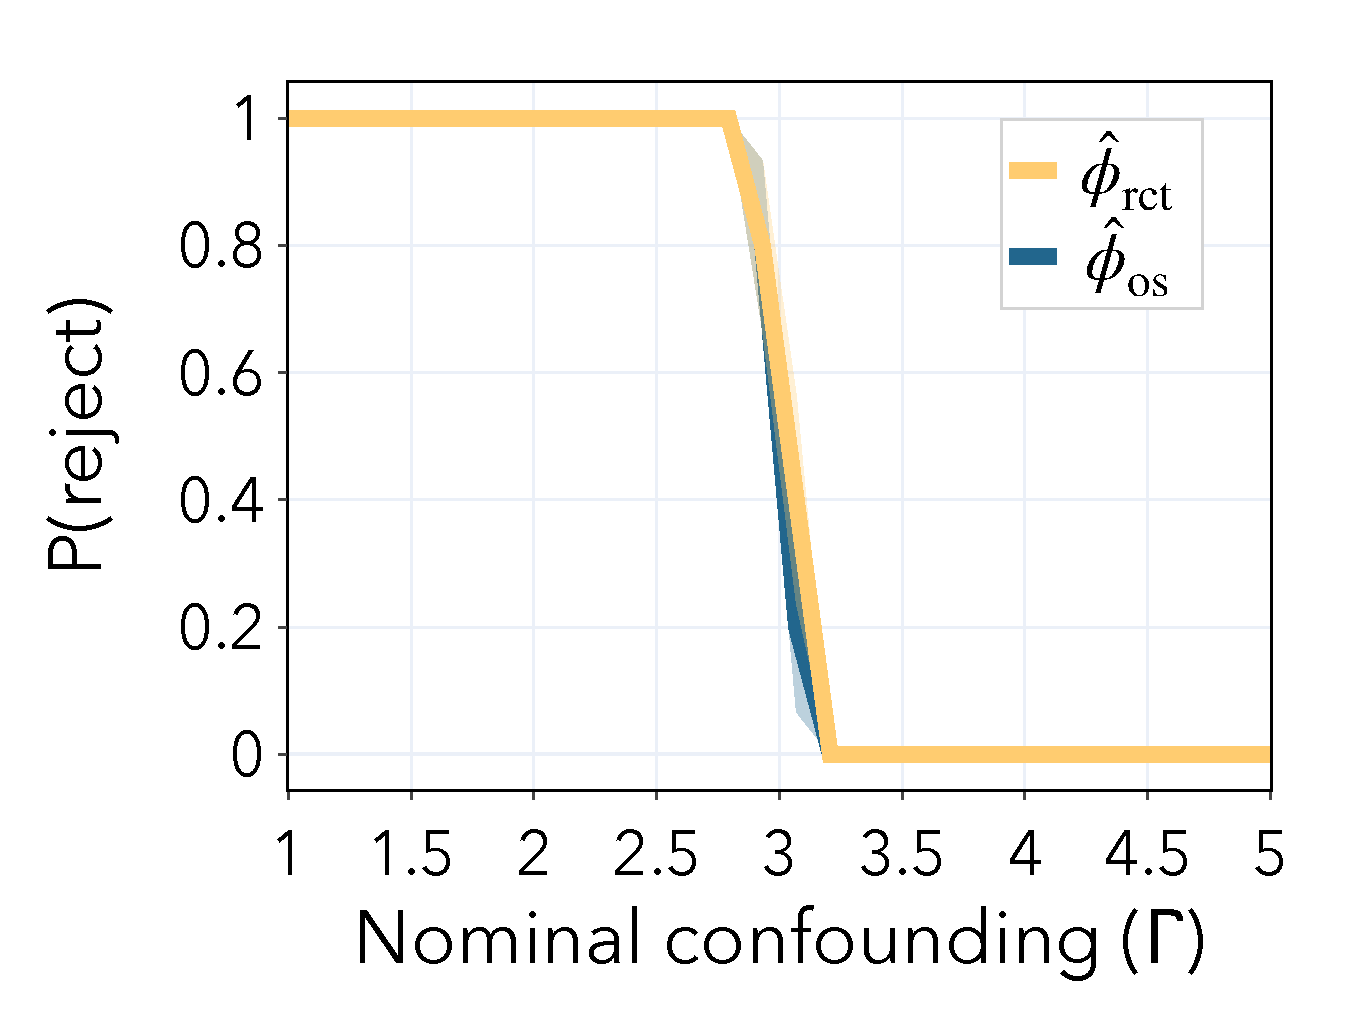
\includegraphics[width=\textwidth]{papers/confounding_test/figures/vote_weak_small.pdf}
    \caption{Weak, small sample}
    \label{fig:confounding-vote-weak-small}
  \end{subfigure}
  \hfill
  \begin{subfigure}[t]{0.46\textwidth}
    \centering
    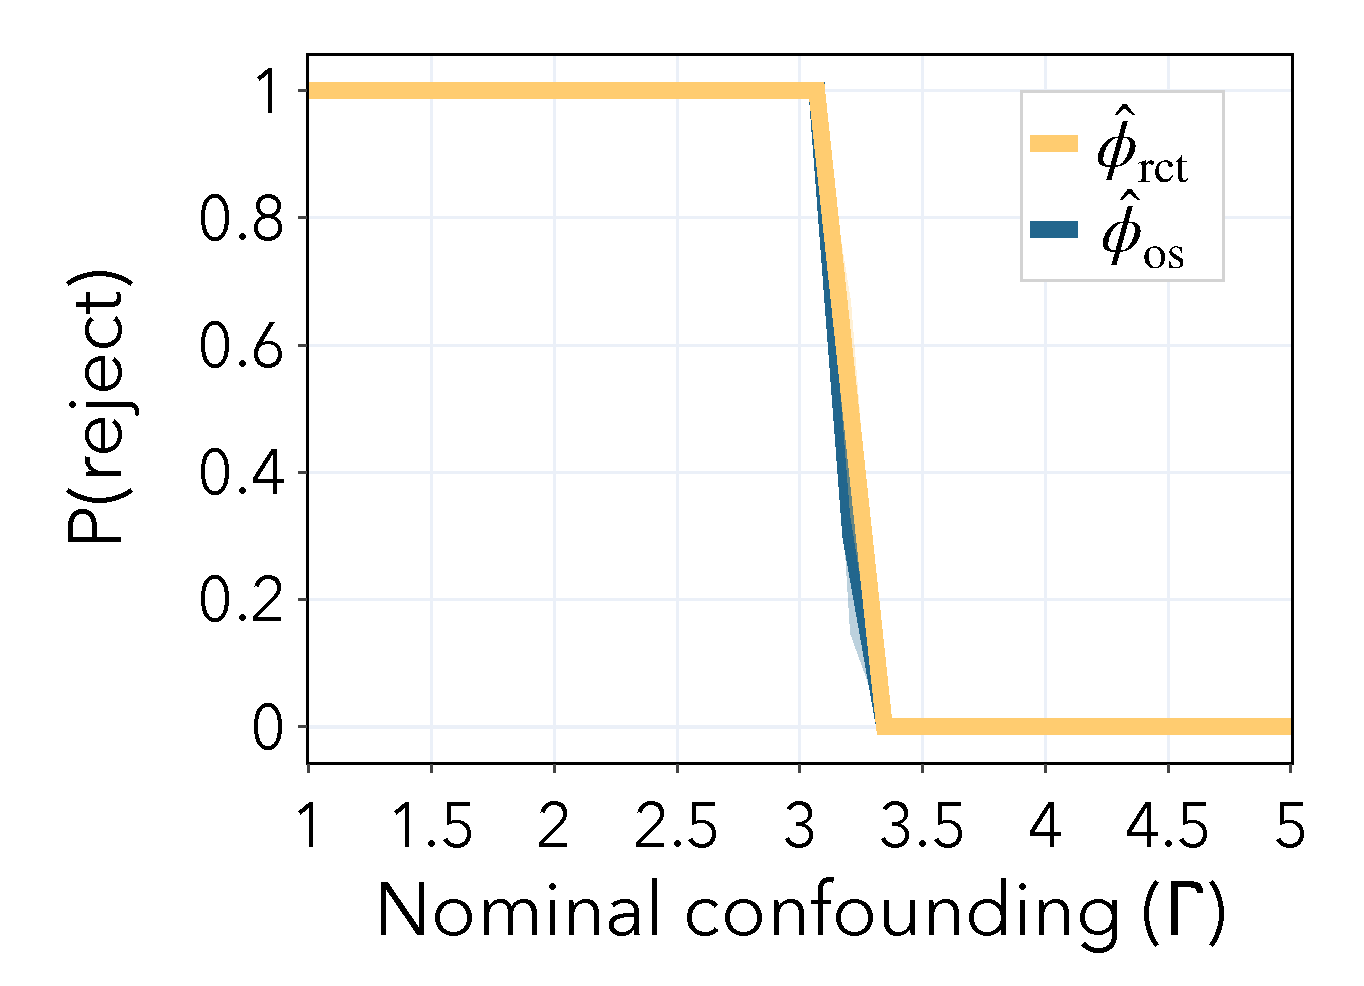
\includegraphics[width=\textwidth]{papers/confounding_test/figures/vote_weak.pdf}
    \caption{Weak, large sample}
    \label{fig:confounding-vote-weak-large}
  \end{subfigure}\\[0.75ex]
  \begin{subfigure}[t]{0.46\textwidth}
    \centering
    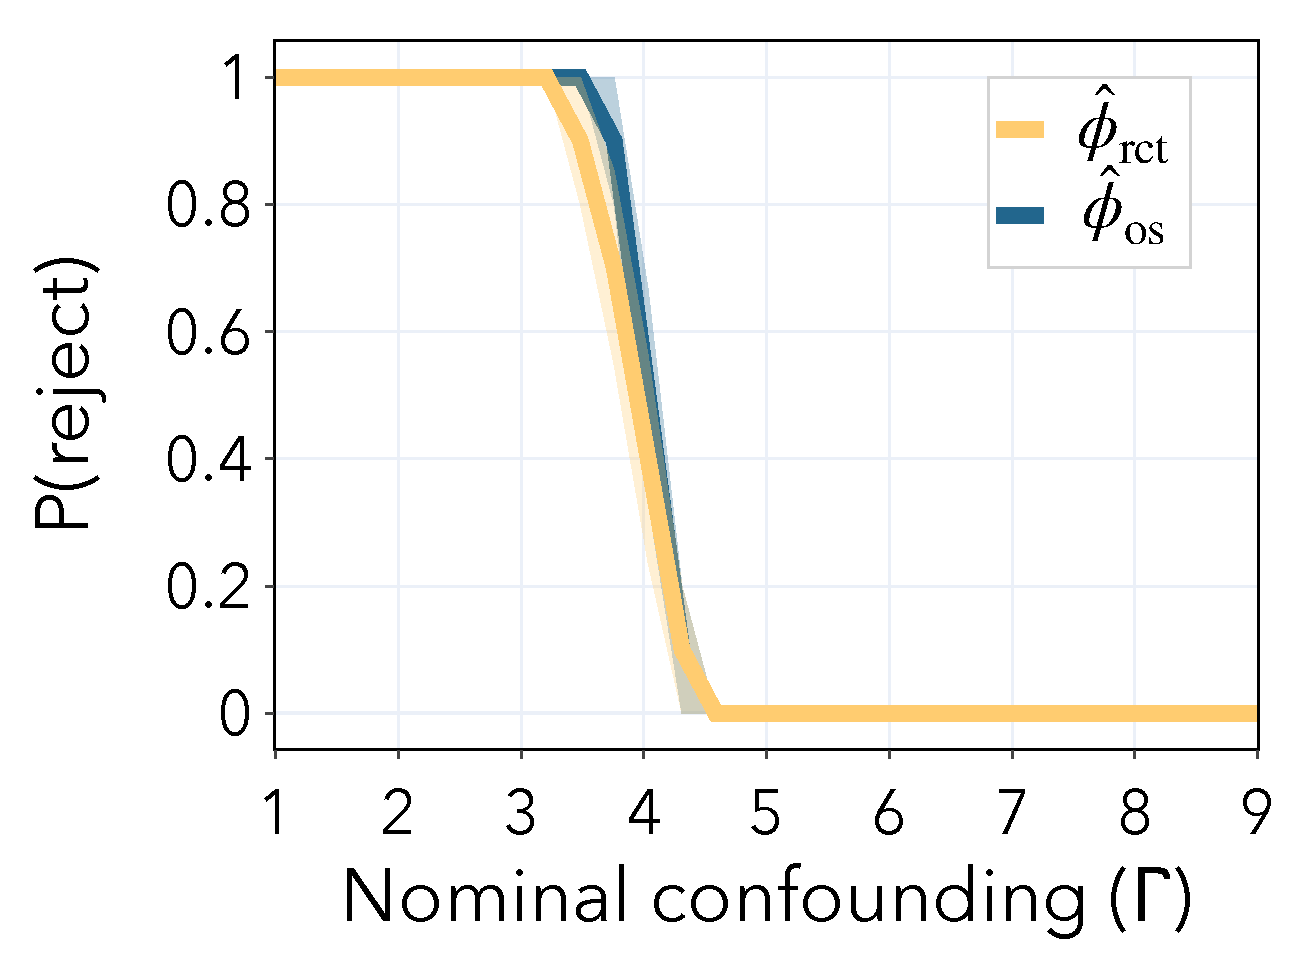
\includegraphics[width=\textwidth]{papers/confounding_test/figures/vote_strong_small.pdf}
    \caption{Strong, small sample}
    \label{fig:confounding-vote-strong-small}
  \end{subfigure}
  \hfill
  \begin{subfigure}[t]{0.46\textwidth}
    \centering
    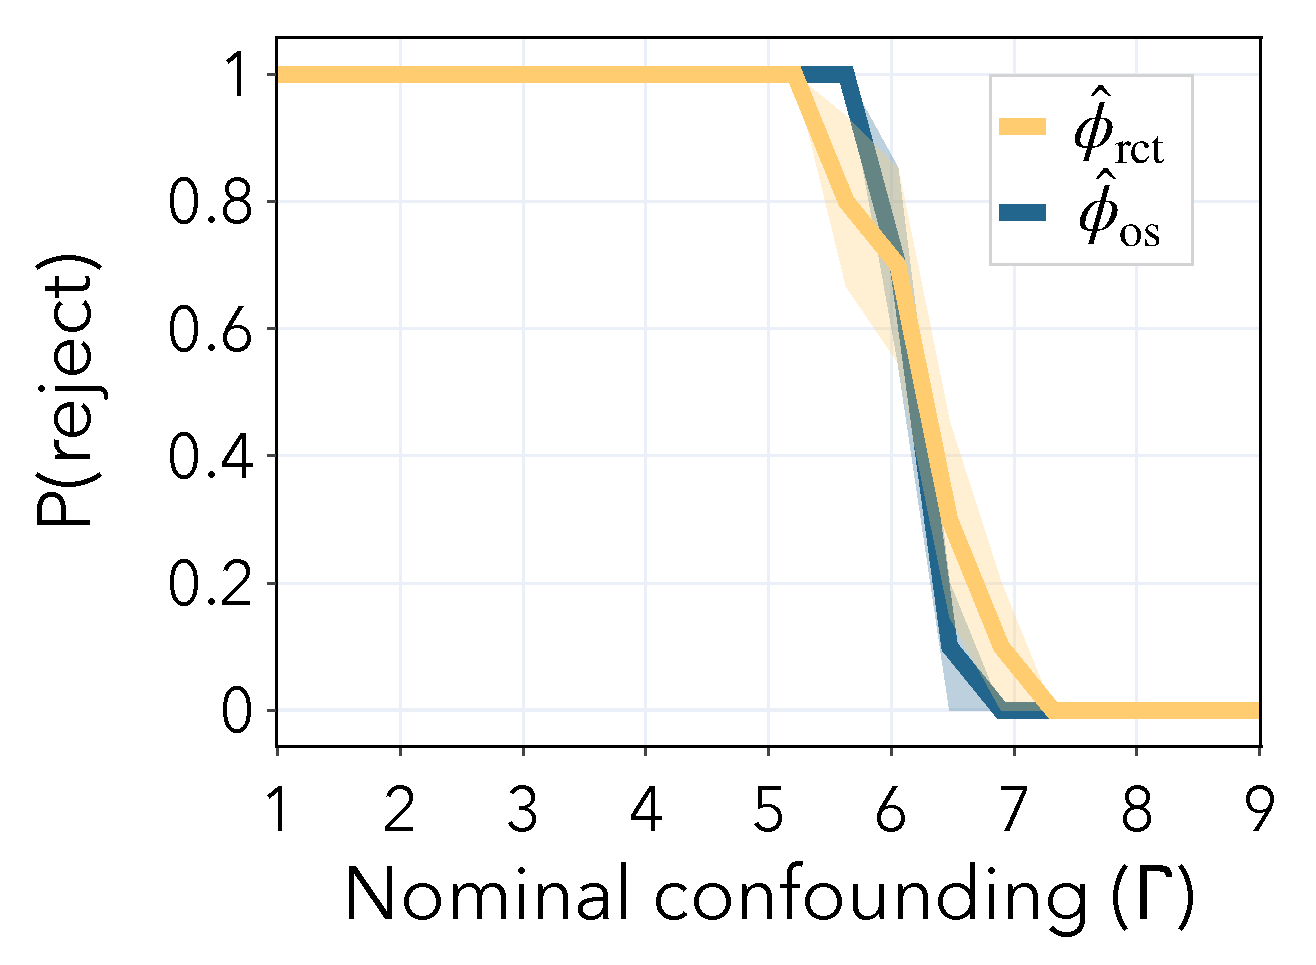
\includegraphics[width=\textwidth]{papers/confounding_test/figures/vote_strong.pdf}
    \caption{Strong, large sample}
    \label{fig:confounding-vote-strong-large}
  \end{subfigure}
  \caption{VOTE rejection probabilities over candidate values of \(\Gamma\), with \(\alpha=0.05\) and \(\Gamma^\star=9\). Small-sample panels use \(n_{\mathrm{rct}}=3{,}200,n_{\mathrm{os}}=11{,}000\); large-sample panels use \(n_{\mathrm{rct}}=10{,}650,n_{\mathrm{os}}=36{,}800\). Panels~(a) and~(b) display \(\Gamma\in[1,5]\) because rejection reaches zero well below \(\Gamma^\star=9\). In the plot legends, \(\hat{\phi}_{\mathrm{os}}\) denotes \(\widehat{\phi}_{\widetilde{\mathrm{os}}}\).}
  \label{fig:confounding-vote-results}
\end{figure}

\subsection{Tennessee STAR Project}
\label{app:confounding-star}

Figure~\ref{fig:confounding-star-results} reports the additional semi-synthetic experiments based on the Tennessee STAR project. Because the dataset is already in a small-sample regime, the comparison focuses on weak versus strong hidden confounders using the original sample sizes. The weak confounder is free-lunch status, and the strong confounder is the outcome \(Y\).

\begin{figure}[!htbp]
  \centering
  \begin{subfigure}[t]{0.46\textwidth}
    \centering
    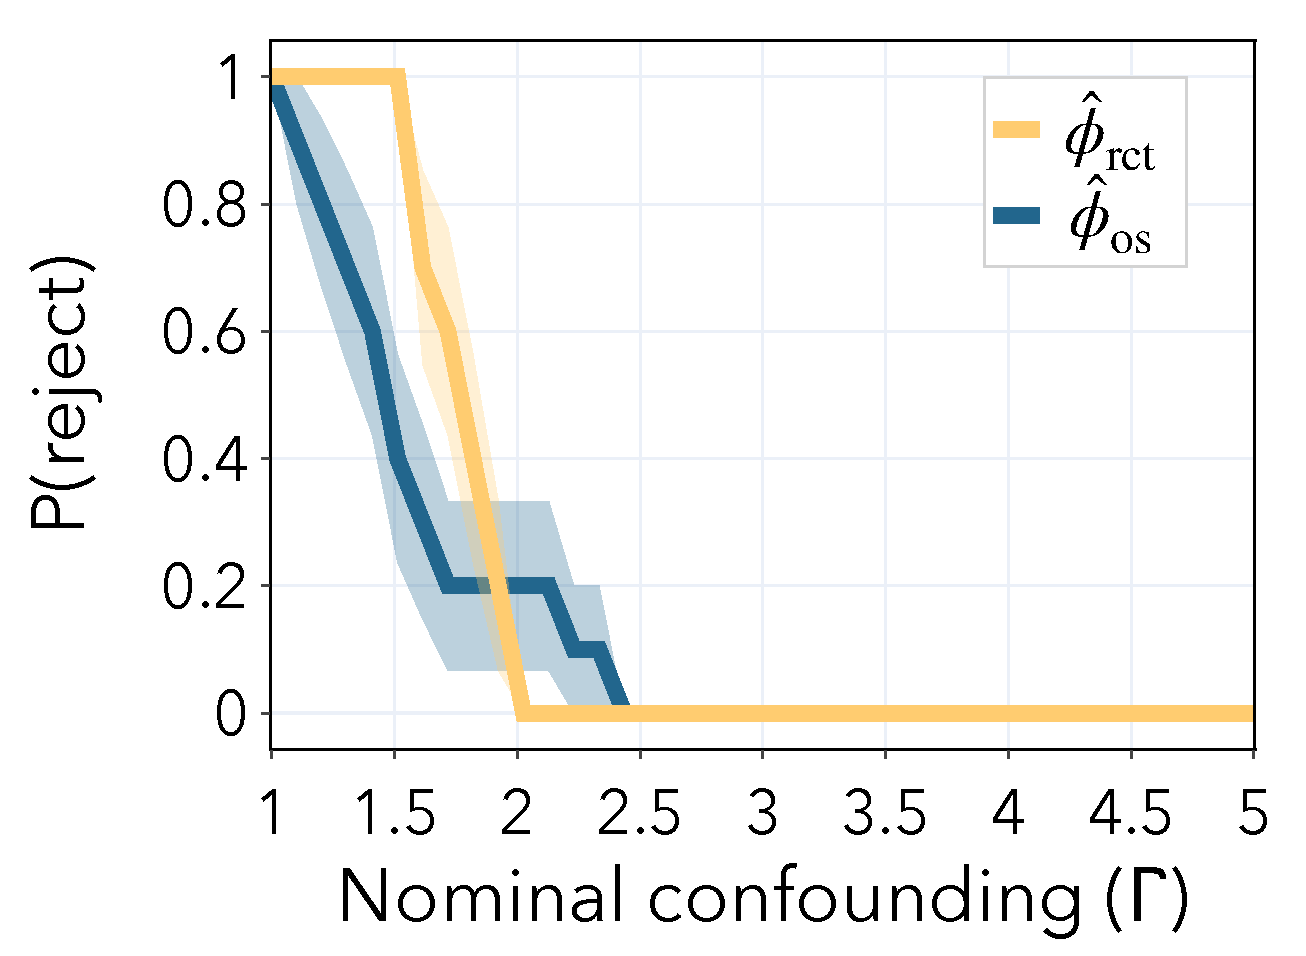
\includegraphics[width=\textwidth]{papers/confounding_test/figures/star_weak.pdf}
    \caption{Weak confounder}
    \label{fig:confounding-star-weak}
  \end{subfigure}
  \hfill
  \begin{subfigure}[t]{0.46\textwidth}
    \centering
    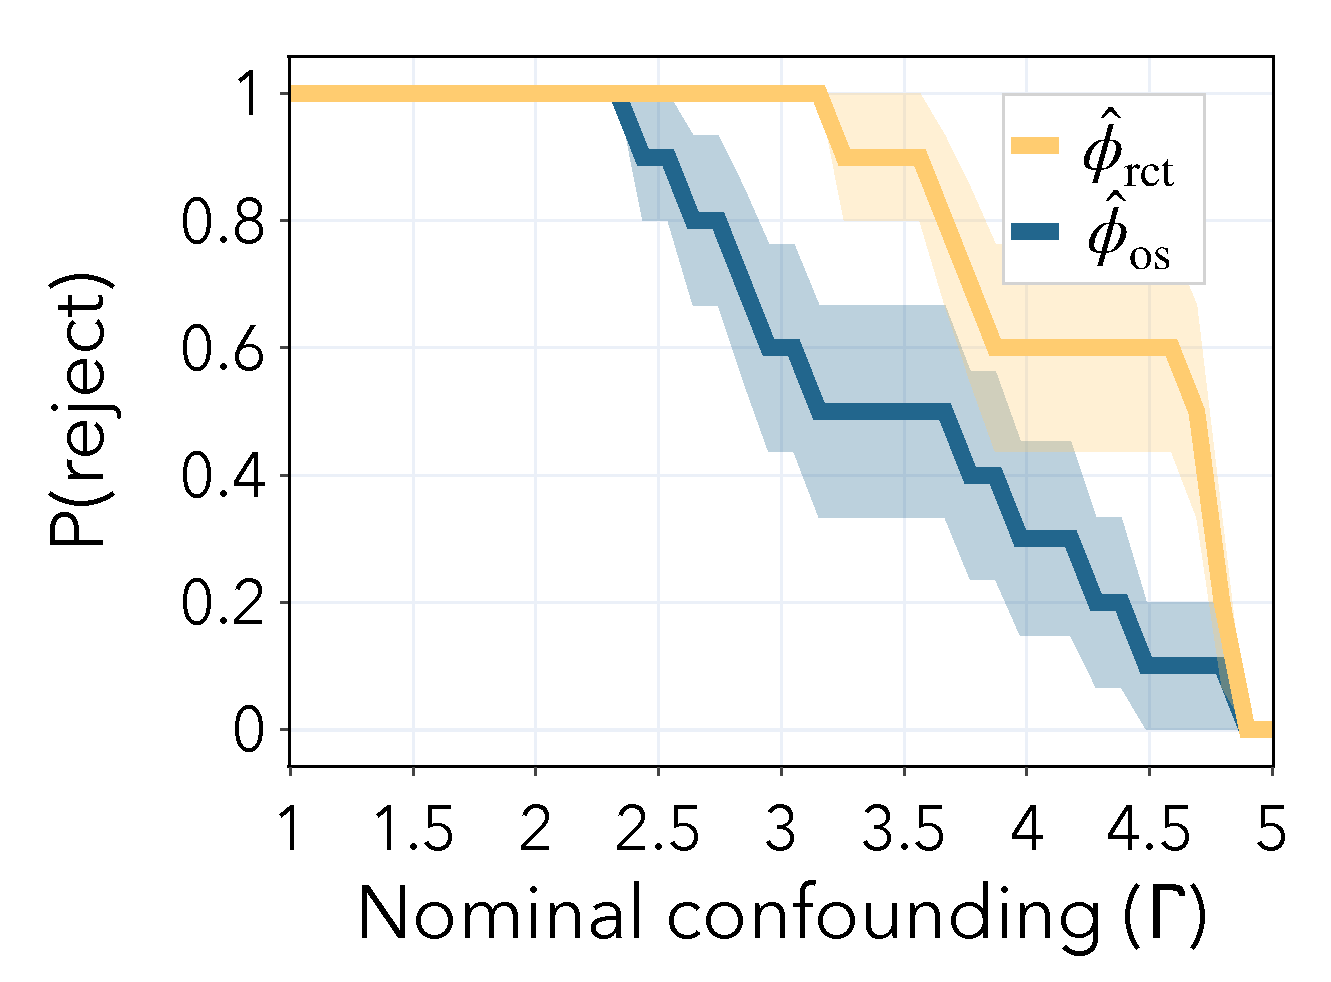
\includegraphics[width=\textwidth]{papers/confounding_test/figures/star_strong.pdf}
    \caption{Strong confounder}
    \label{fig:confounding-star-strong}
  \end{subfigure}
  \caption{Tennessee STAR rejection probabilities over candidate values of \(\Gamma\), with \(\alpha=0.05\), \(\Gamma^\star=5\), \(n_{\mathrm{rct}}=600\), and \(n_{\mathrm{os}}=1{,}800\). In the plot legends, \(\hat{\phi}_{\mathrm{os}}\) denotes \(\widehat{\phi}_{\widetilde{\mathrm{os}}}\).}
  \label{fig:confounding-star-results}
\end{figure}
